\documentclass[a4paper,kulak]{kulakarticle} %options: kul or kulak (default)

\usepackage[dutch]{babel}
\usepackage{amsmath}
\usepackage{tikz}
% TikZ Stuffs
\tikzset{every label/.style={font=\footnotesize,inner sep=1pt}}
\newcommand{\stencilpt}[4][]{\node[circle,fill,draw,inner sep=1.5pt,label={above left:#4},#1] at (#2) (#3) {}}
% End of TikZ Stuffs
\usepackage{listings}
% Let's hope this works
\newcommand{\inputcode}[1]{
	\lstinputlisting[language=Octave]{C:/Users/diete/Documents/Uni Docs/Numerieke Wiskunde/PracHeatEquation/Coding/#1.m}
}
\usepackage{appendix}
\usepackage{float}
\usepackage{url}

\date{Academiejaar 2021 -- 2022}
\address{
  Bachelor Informatica \\
  Numerieke Wiskunde \\
  Koen Van Den Abeele / Nithin Govindarajan}
\title{Practicum: De Warmtevergelijking}
\author{Dieter Demuynck}


\begin{document}

\maketitle

\section*{Inleiding}

De warmtevergelijking is een redelijk gekende vergelijking in de fysica. Hij kan worden geschreven als

\begin{equation}
	\frac{\partial u(\vec{x}, t)}{\partial t} = \alpha \Delta u(\vec{x}, t)
\end{equation}

waarbij $u(\vec{x}, t)$ de temperatuurverdeling op een positie $\vec{x} \in \Omega$ met $\Omega$ een domein, een tijdsinterval $t \in [0, T]$, de diffusiviteit en $\Delta$ de Laplaciaan is. Deze vergelijking wordt gebruikt om de diffusie van warmte in de ruimte en tijd te berekenen aan de hand van begin- en randvoorwaarden.  % TODO: Complete explanation

\section{Warmtevergelijking in 1D}

\subsection{De vergelijking opstellen}
De één-dimensionale warmtevergelijking $u(x, t)$ kan gebruikt worden om de warmte te berekenen in simpele objecten, zoals een staaf. Om deze warmtevergelijking op te stellen, wordt de wet van Fourier gebruikt. % TODO: Reference!!!
De wet van Fourier beweert dat de snelheid van de stroming van warmte per oppervlakte-eenheid $\vec{q}$, een vectorveld, door een oppervlakte proportioneel is met min de gradiënt van de warmteverdeling $u(\vec{x}, t)$. Dit geeft de vergelijking

\begin{equation}
	\vec{q} = - k \nabla u
\end{equation}

waarbij k de warmtegeleidingscoëfficiënt is.
In een één-dimensionaal stelsel wordt de positie voorgesteld door 1 coördinaat $x$, waardoor $q(x, t)$ een scalair veld wordt en de gradiënt $\nabla u (x, t)$ simpelweg een afgeleide naar $x$ wordt. Dus  wordt de vergelijking

\begin{equation*}
	q = -k\frac{\partial u}{\partial x}
\end{equation*}

We definiëren nu ook de functie $Q(x, t)$ dat de interne warmte energie per eenheid volume van de staaf beschrijft op elk punt $x$ op tijdstip $t$. Wanneer er geen warmte wordt toegevoegd aan het systeem, is de snelheid van de verandering van de interne warmte energie per volume-eenheid $Q$ proportioneel met de snelheid van de verandering van de temperatuur $u$. Wanneer van een constante dichtheid en warmte capaciteit wordt uitgegaan, geldt dat

\begin{equation}
	\frac{\partial Q}{\partial t} = c \rho \frac{\partial u}{\partial t}
\end{equation}

waarbij $c$ de specifieke warmte capaciteit en $\rho$ de dichtheid van het materiaal. 
Wanneer hierop de wet van behoud van energie wordt toegepast op een klein gebied rond elk punt x, concludeert men dat de afgeleide van $Q$ naar $t$ gelijk is aan min de afgeleide van $q$ naar $x$. In symbolen:

\begin{equation*}
	\frac{\partial Q}{\partial t} = - \frac{\partial q}{\partial x}
\end{equation*}

waaruit volgt dat

\begin{equation*}
	\begin{split}
	\frac{\partial u}{\partial t} &= - \frac{1}{c\rho} \frac{\partial q}{\partial x} \\
	&= - \frac{1}{c\rho} \frac{\partial}{\partial x} 
		\left( - k \frac{\partial u}{\partial x} \right) \\
	&= \frac{k}{c\rho} \frac{\partial^2u}{\partial x^2}
	\end{split}
\end{equation*}

Stellen we $\alpha = \frac{k}{c \rho}$ geeft dit de warmtevergelijking in 1 dimensie

\begin{equation}
	\frac{\partial u(x, t)}{\partial t} = \alpha \frac{\partial^2u(x, t)}{\partial x^2}
	\label{eq:1D_heat}
\end{equation}

Hierbij noemt $\alpha$ de warmtediffusiviteit. % TODO: Understand wtf is going on...

\subsection{Expliciete numerieke simulatie}

Om de één-dimensionale warmtevergelijking numeriek op te lossen zullen we gebruik maken van de formules voor voorwaartse differenties, en centrale differenties voor equidistante punten, elk voor de afgeleide in de tijd respectievelijk voor de (tweede) afgeleide in de ruimte. % TODO: Reference book p136
We noemen deze methode expliciet wegens de manier waarop we elke waarde op een volgend tijdstip berekenen. Uiteindelijk bekomen we een formule van de vorm % TODO: reference wikipedia explicit vs implicit

\begin{equation*}
	Y(t + \Delta t) = F(Y(t))
\end{equation*}

We gebruiken de notatie $u_i^n = u(x_i, t_n)$ waarbij $x_i = i\Delta x$ voor $i = 0, 1, ..., N_x-1$ en $t_n = n\Delta t$ waarbij $n = 0, 1, ..., N_t - 1$. Hierbij is $N_x$ en $N_t$ het aantal waarden voor $x$ resp. $t$.
Dan geldt:

\begin{equation}
	\partial_t u_i^n = \frac{u_i^{n+1} - u_i^n}{\Delta t} + O(\Delta t)
	\label{eq:diff_time}
\end{equation}

\begin{equation}
	\partial_{xx} u_i^n = \frac{u_{i-1}^n - 2 u_i^n + u_{i+1}^n}{(\Delta x)^2} + O((\Delta x)^2)
	\label{eq:diff_space}
\end{equation}

Deze formules zullen benaderend gelijk zijn na het weglaten van de termen binnenin de O-notatie. Die benaderende formules invullen in de warmtevergelijking \ref{eq:1D_heat} geeft dan:

\begin{align*}
	\frac{u_i^{n+1} - u_i^n}{\Delta t} &\approx \alpha \frac{u_{i-1}^n - 2 u_i^n + u_{i+1}^n}{(\Delta x)^2} \\
	\Leftrightarrow \qquad u_i^{n+1} &\approx \frac{\alpha \Delta t}{(\Delta x)^2} u_{i-1}^n + \left( 1 - \frac{2 \alpha \Delta t}{(\Delta x)^2} \right) u_i^n + \frac{\alpha \Delta t}{(\Delta x)^2} u_{i+1}^n 
\end{align*}

Stel $r = \frac{\alpha \Delta t}{(\Delta x)^2}$, dan is deze vergelijking makkelijker te schrijven als

\begin{equation}
	u_i^{n+1} \approx r u_{i-1}^n + \left( 1 - 2r \right) u_i^n + r u_{i+1}^n 
	\label{eq:expl_recursive}
\end{equation}

\begin{figure}
\centering
\begin{tikzpicture}[scale=2]
	\stencilpt[red]{-1, 0}{i-1}{$u_{i-1}^n$};
	\stencilpt[red]{0, 0}{i}{$u_i^n$};
	\stencilpt[red]{1, 0}{i+1}{$u_{i+1}^n$};
	\stencilpt{0, 1}{j+1}{$u_i^{n+1}$};
	
	\draw (i-1) -- (i)
	(i)	-- (i+1)
	(i)	-- (j+1);
\end{tikzpicture}
\label{fig:stencil_explicit}
\caption{Stencil voor het berekenen van een waarde $u_i^{n+1}$ op een volgend tijdstip met index n+1 met behulp van de expliciete methode}
\end{figure}

Dit is een formule om de warmte op een punt x op volgend tijdstip te berekenen aan de hand van de warmte in het punt x, links van x en recht van x op het huidig tijdstip. Figuur \ref{fig:stencil_explicit} geeft een grafische voorstelling van deze bewerking onder de vorm van een stencil. \\
Deze recursieve formule kan worden genoteerd als een matrix matrixvermenigvuldiging
\begin{equation}
	% MATRIX T
	\begin{bmatrix}
		\qquad \\
		T \\
		\\ 
	\end{bmatrix}
	% CURRENT VERTEX
	\begin{bmatrix}
		u_0^n \\
		\vdots \\
		u_{N_x - 1}^n
	\end{bmatrix}
	=
	% NEXT VERTEX
	\begin{bmatrix}
		u_0^{n+1} \\
		\vdots \\
		u_{N_x - 1}^{n+1}
	\end{bmatrix}	
\end{equation}

Hierbij is $T$ een matrix waarbij de diagonaalelementen gelijk zijn aan $1-2r$ en alle elementen net boven en onder de diagonaal zijn dan gelijk aan $r$. Alle andere elementen zijn gelijk aan nul. Dit soort matrices, met elementen verschillend van nul op, boven en onder de diagonaal met alle andere elementen gelijk aan nul, noemen we een \textit{tridiagonaal matrix}.

\begin{equation}
	\begin{bmatrix}
		\qquad \\
		T \\
		\\ 
	\end{bmatrix}
	=
	\begin{bmatrix}
		1-2r	&	r		&	0		&	\dots	&	0 		\\
		r		&	1-2r	&	r		&	\dots	&	0		\\
		0		&	r		&	1-2r	&	\dots	&	0		\\
		\vdots	&	\vdots	&	\vdots	&	\ddots	&	\vdots	\\
		0		&	0		&	0		&	\dots	&	1-2r	\\
		\\ 
	\end{bmatrix}
\end{equation}

Merk op dat er een probleem optreed bij de randwaarden, waar $i = 0$ en $i = N_x-1$. Om bijvoorbeeld $u_0^{n+1}$ te berekenen, zijn er waarden nodig die buiten het toegelaten interval voor x liggen. Echter is dit geen probleem, aangezien deze elementen gekend zijn door de opgelegde randvoorwaarden en hoeven ze dus niet berekend te worden a.d.h.v. de recursieformule.

\subsubsection{Implementatie bij constante randvoorwaarden}
\label{sec:implementatie_expliciet_constant}

De implementatie \path{heat_explicit.m} (zie Appendix \ref{code:heat_explicit}) voor het numeriek berekenen van de warmtevergelijking in 1D werkt als volgt: \\
De lengte van de staaf, de tijd tot wanneer we de warmteverspreiding willen simuleren en het aantal stappen, samen met de diffusiviteit van de staaf worden allen ingegeven als constanten. De constante randvoorwaarde $u = T_{om}$ wordt gevraagd voor positie $x = L$ voor alle $t \in [0, T]$, en op positie $x = 0$ wordt ervan uitgegaan dat daar de constante randvoorwaarde $u = 0$ geldt voor alle $t \in [0, T]$. De beginvoorwaarden worden niet rechtstreeks meegegeven, maar eerder als een aparte functie \path{initval(x)} die bij het document zit. Er wordt gevraagd dat deze functie de positie $x$ afbeeldt op de begintemperatuur van de staaf op die positie. De functie \path{heat_explicit} zal zelf de randvoorwaarden gebruiken om de initiële waarden te overschrijven, zodat de gebruiker niet per se een functie moet opstellen die aan deze randvoorwaarden voldoet.

\subsubsection{Implementatie bij convectie-randvoorwaarde}

Stel dat op $x = 0$ de randvoorwaarde een convectie vergelijking is, zoals

\begin{equation}
	\frac{\partial u(0, t)}{\partial x} = \frac{H}{K}\left[u(0, t) - T_{omgeving}\right]
	\label{eq:convection_term}
\end{equation}

Bij het toepassen van centrale differenties op de afgeleide in bovenstaande vergelijking geldt:

\begin{equation*}
	\partial_x u_0^n \approx \frac{u_1^n - u_{-1}^n}{2(\Delta x)^2}
\end{equation*}

waardoor

\begin{align*}
	\frac{u_1^n - u_{-1}^n}{2(\Delta x)^2} &\approx \frac{H}{K}\left[u(0, t) - T_{omgeving}\right] \\
	\Leftrightarrow \qquad
	u_{-1}^n &\approx 
	\frac{2 H (\Delta x)^2}{K} T_{omgeving} 
	- \frac{2 H (\Delta x)^2}{K} u_0^n
	+ u_1^n
\end{align*}

Stel $q = \frac{2 H (\Delta x)^2}{K}$, dan is de vergelijking te schrijven als

\begin{equation}
	u_{-1}^n \approx q T_{omgeving} - q u_0^n + u_1^n
	\label{eq:convection_diff}
\end{equation}

Als we formule \ref{eq:expl_recursive} toepassen op $u_0^n$ bekomen we

\begin{equation*}
	u_0^{n+1} \approx r u_{-1}^n + \left( 1 - 2r \right) u_0^n + r u_1^n 
\end{equation*}

Wanneer we daarin vergelijking \ref{eq:convection_diff} toepassen, resulteert dit in

\begin{align*}
	u_0^{n+1} 
	&\approx r \left(q T_{omgeving} - q u_0^n + u_1^n\right) 
	+ \left( 1 - 2r \right) u_0^n 
	+ r u_1^n \\
	&\approx 2 r u_1^n
	+ ( - q r + 1 - 2 r ) u_0^n
	+ r q T_{omgeving} \\
	&\approx 2 r u_1^n
	+ (1 - (2 + q)r) u_0^n
	+ r q T_{omgeving}
\end{align*}

Door gebruik te maken van de beginvoorwaarde in $u(0, 0)$ kunnen we zo dus recursief de temperatuur op een volgend tijdstip op positie 0 berekenen. Door de eerste twee elementen op de eerste rij van de matrix $T$ aan te passen naar $(1 - (2 + q)r)$ voor het eerste element en $2r$ voor het tweede, deze matrix te vermenigvuldigen met de temperatuurvector op het huidig tijdstip, en daarna bij het eerste element (wat de temperatuur op positie $x = 0$ op een volgend tijdstip voorstelt) nog $r q T_{omgeving}$ op te tellen, bekomen we onmiddellijk de correcte temperatuur. \\
De implementatie met de convectieterm zal dan ook verschillen met de implementatie bij constante randvoorwaarden \ref{code:heat_explicit}(zie sectie \ref{sec:implementatie_expliciet_constant}) enkel en alleen bij de stappen uitgelegd in vorige paragraaf. De code voor deze implementatie is te vinden in appendix \ref{code:convheat_explicit}.

\subsection{Impliciete numerieke simulatie}

Naast de expliciete methode zoals eerder vermeld is er ook een impliciete methode om de waarden op een volgend tijdstip te berekenen. Deze methode geeft ons dan een vergelijking van de vorm

\begin{equation*}
	G(Y(t + \Delta t), Y(t)) = 0
\end{equation*}

Om deze vergelijk op te stellen gebruiken we centrale differenties voor de (tweede) afgeleide in beide tijd en ruimte in de warmtevergelijking \ref{eq:1D_heat}. We discretiseren de vergelijking telkens op halve tijdstippen $t = (j + 1/2) \Delta t$, waardoor de centrale differenties voor de tijdsafgeleide steeds hele tijdstippen $t = \Delta t$ gebruikt. Dit zorgt echter voor problemen voor de differenties van de ruimtelijke afgeleide, aangezien we geen waarden hebben voor deze halve tijdstippen. Om deze waarden te benaderen gebruiken we de methode van Lax, die deze benadering berekend door het gemiddelde te nemen van de aangrenzende waarden:

\begin{equation}
	u_i^{t + 1/2} \approx \frac{u_i^t + u_i^{t + 1}}{2}
	\label{eq:lax_method}
\end{equation}

De centrale differenties voor de afgeleiden geeft dan volgende vergelijkingen

\begin{align*}
	\partial_t u_i^{n+\frac{1}{2}} 
	&= \frac{u_i^{n+1} - u_i^n}{2\Delta t} + O((\Delta t)^2)
\end{align*}

\begin{align*}
	\partial_{xx} u_i^{n+\frac{1}{2}} 
	&= \frac{u_{i-1}^{n+\frac{1}{2}} - 2 u_i^{n+\frac{1}{2}} + u_{i+1}^{n+\frac{1}{2}}}{(\Delta x)^2} + O((\Delta x)^2) \\
	&= \frac{u_{i-1}^{n+1} - 2 u_i^{n+1} + u_{i+1}^{n+1} + u_{i-1}^n - 2 u_i^n + u_{i+1}^n}{2(\Delta x)^2} + O((\Delta x)^2)
\end{align*}

Deze formules ingeven in de warmtevergelijking \ref{eq:1D_heat} en de hogere orde termen te verwaarlozen resulteert in:

\begin{equation*}
	\frac{u_i^{n+1} - u_i^n}{\Delta t}
	\approx
	\alpha \frac{u_{i-1}^{n+1} - 2 u_i^{n+1} + u_{i+1}^{n+1} + u_{i-1}^n - 2 u_i^n + u_{i+1}^n}{(\Delta x)^2}
\end{equation*}

Stel $r = \frac{\alpha \Delta t}{(\Delta x)^2}$, dan is deze vergelijking gelijk aan

\begin{equation}
	- r u_{i-1}^{n+1}
	+ \left(1 + 2r\right) u_i^{n+1}
	- r u_{i+1}^{n+1}
	\approx
	r u_{i-1}^n
	+ \left(1 - 2 r\right) u_i^n
	+ r u_{i+1}^n
	\label{eq:implicit_recursive}
\end{equation}

\begin{figure}
	\centering
	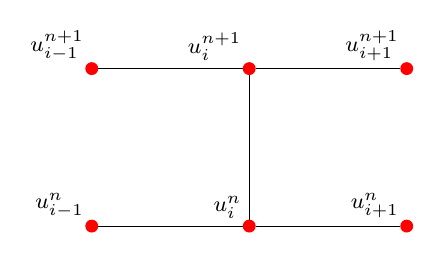
\begin{tikzpicture}[scale=2]
		\stencilpt[red]{-1, 0}{i-1}{$u_{i-1}^n$};
		\stencilpt[red]{0, 0}{i}{$u_i^n$};
		\stencilpt[red]{1, 0}{i+1}{$u_{i+1}^n$};
		\stencilpt[red]{-1, 1}{i-1 j+1}{$u_{i-1}^{n+1}$};
		\stencilpt[red]{0, 1}{j+1}{$u_i^{n+1}$};
		\stencilpt[red]{1, 1}{i+1 j+1}{$u_{i+1}^{n+1}$};
		
		\draw (i-1) -- (i)
		(i)	-- (i+1)
		(i)	-- (j+1)
		(j+1) --  (i-1 j+1)
		(j+1) -- (i+1 j+1);
	\end{tikzpicture}
	\label{fig:stencil_implicit}
	\caption{Stencil voor het berekenen van een waarde $u_i^{n+1}$ op een volgend tijdstip met index n+1 met behulp van de impliciete methode}
\end{figure}

Een grafische voorstelling van de waarden die worden gebruikt tijdens elke berekening is te vinden op figuur \ref{fig:stencil_implicit}. \\
De vergelijking kunnen we ook in matrixvorm schrijven als

\begin{equation}
	% MATRIX T
	\begin{bmatrix}
		\qquad \\
		A \\
		\\ 
	\end{bmatrix}
	% CURRENT VERTEX
	\begin{bmatrix}
		u_0^{n+1} \\
		\vdots \\
		u_{N_x - 1}^{n+1}
	\end{bmatrix}
	=
	% NEXT VERTEX
	\begin{bmatrix}
		b_0^n \\
		\vdots \\
		b_{N_x - 1}^n
	\end{bmatrix}
	\label{eq:impl_matrix}	
\end{equation}

waarbij

\begin{equation*}
	\begin{bmatrix}
		\qquad \\
		A \\
		\\ 
	\end{bmatrix}
	=
	\begin{bmatrix}
		1+2r	&	-r		&	0		&	\dots	&	0 		\\
		-r		&	1+2r	&	-r		&	\dots	&	0		\\
		0		&	-r		&	1+2r	&	\dots	&	0		\\
		\vdots	&	\vdots	&	\vdots	&	\ddots	&	\vdots	\\
		0		&	0		&	0		&	\dots	&	1+2r	\\
		\\ 
	\end{bmatrix}
\end{equation*}

en

\begin{equation*}
	b_i^n = (1-2r)u_i^n + r(u_{i-1}^n + u_{i+1}^n)
\end{equation*}

Merk weer op dat dit problemen veroorzaakt op de rand van het ruimtelijk interval, maar opnieuw zal dit niet belangrijk zijn dankzij de opgelegde randvoorwaarden. 

\subsubsection{Implementatie bij constante randvoorwaarden}
\label{sec:implementatie_impliciet_constant}

Om de waarden $u_i^{n+1}$ uit formule \ref{eq:impl_matrix} te bereken moet een stelsel opgelost worden. Dit maakt het moeilijker om de randvoorwaarden toe te passen tijdens de implementatie: de waarden tussen de randen op een volgend tijdstip zijn nu ook afhankelijk van de waarden op de randen op dit volgend tijdstip. In de expliciete methode\ref{sec:impl_expl_constant} was dit niet het geval, daar konden we de randwaarden simpelweg overschrijven met de opgelegde randvoorwaarden na de berekeningen. \\
Het stelsel zal lichtjes moeten aangepast worden om de randvoorwaarden toe te passen tijdens de berekeningen. Aangezien we uitgaan van constante randvoorwaarden $u(0, t) = 0$ en $u(L, t) = T_{omgeving}$, kunnen we dit noteren in het stelsel door de eerste rij en de laatste rij in de matrix $A$ te vervangen door
$\big(\begin{smallmatrix}
	1 & 0 & 0 & \dots & 0
\end{smallmatrix}\big)$ 
respectievelijk
$\big(\begin{smallmatrix}
	0 & \dots & 0 & 0 & 1
\end{smallmatrix}\big)$
. Daarbij kunnen we dan $b_0^n$ en $b_{N_x - 1}^n$ gelijkstellen aan $0$ respectievelijk $T_{omgeving}$. Daarna hoeven we enkel een stelsel op te lossen. Dit doen we door de ingebouwde functie \path{rref(A)} van \textit{MatLab} toe te passen op de uitgebreide matrix, en de laatste kolom te beschouwen.

\subsubsection{Implementatie bij convectie-randvoorwaarde}

Stel dat we in formule \ref{eq:implicit_recursive} weer $i = 0$ stellen. Dan bekomen we

\begin{equation*}
	- r u_{-1}^{n+1}
	+ \left(1 + 2r\right) u_0^{n+1}
	- r u_1^{n+1}
	\approx
	r u_{-1}^n
	+ \left(1 - 2 r\right) u_0^n
	+ r u_1^n
\end{equation*}

We kunnen dan formule \ref{eq:convection_diff} toepassen om de termen met $i = -1$ om te vormen naar waarden die we wel kennen of kunnen berekenen:

\begin{align*}
	- r \left(q T_{omgeving} - q u_0^{n+1} + u_1^{n+1}\right)
	+ \left(1 + 2r\right) u_0^{n+1}
	- r u_1^{n+1}
	&\approx
	r \left(q T_{omgeving} - q u_0^n + u_1^n\right)
	+ \left(1 - 2 r\right) u_0^n
	+ r u_1^n \\
	\Leftrightarrow \qquad
	\left(1 + r (2 + q)\right) u_0^{n+1}
	- 2 r u_1^{n+1}
	&\approx
	\left(1 - r (2 + q)\right) u_0^n
	+ 2 r u_1^n
	+ 2 r q T_{omgeving}
\end{align*}

Waarbij opnieuw $q = \frac{2 H (\Delta x)^2}{K}$.\\*
Door de eerste twee termen in de eerste rij in de matrix A in formule \ref{eq:impl_matrix} te vervangen met de coëfficiënten zoals hierboven beschreven, en de term $b_0^n$ gelijk te stellen aan het rechterlid, kunnen we de convectieterm voor $x=0$ toepassen in de berekeningen. We gebruiken dezelfde methode beschreven in sectie \ref{sec:implementatie_impliciet_constant} voor de randwaarde in $x = L$ en voor het stelsel op te lossen.

\section*{Besluit}

Afsluitende tekst.

\section*{Appendices}

\appendix

\section{Bestand: heat\textunderscore explicit.m}
	\label{code:heat_explicit}
	\inputcode{heat_explicit}

\newpage
\section{Bestand: convheat\textunderscore explicit.m}
	\label{code:convheat_explicit}
	\inputcode{convheat_explicit}
	
\newpage
\section{Bestand: heat\textunderscore implicit.m}
	\label{code:heat_implicit}
	\inputcode{heat_implicit}
	
% \newpage
% \section{File: convheat\textunderscore implicit.m}
% \label{code:convheat_implicit}
% \inputcode{convheat_implicit}
	

\end{document}
